% !TeX root = ../main.tex
% PointWorld, Fig. 16, physical PDF page 33, the first DROID cloth case.
% Both future panels refer to the same 1.0 s horizon and author rendering view.
% Reference annotations are distinct from model predictions; no execution is relabeled.
\begingroup
\linespread{1}\selectfont
\begin{tikzpicture}[
  x=1cm,y=1cm,text=black,line cap=round,line join=round,
  font=\songti\fontsize{10pt}{12pt}\selectfont,
  every node/.style={align=center,outer sep=0pt,inner sep=0pt},
  lpTitle/.style={font=\heiti\fontsize{10.5pt}{13pt}\selectfont},
  lpFrame/.style={draw=black,line width=0.65pt},
  lpPhoto/.style={anchor=north west},
  lpArrow/.style={draw=black,line width=0.8pt,
    -{Latex[length=1.8mm,width=1.2mm]}}
]
  \path[use as bounding box] (0,0) rectangle (16,6.65);
  \foreach \xl/\xr/\xc/\heading in {
    0.10/4.80/2.450/RGB观测（两视角）,
    5.40/10.35/7.875/模型预测,
    10.95/15.90/13.425/参考标注}{%
    \draw[lpFrame] (\xl,0.15) rectangle (\xr,6.50);
    \path[fill=black!5] (\xl+0.01,5.96) rectangle (\xr-0.01,6.49);
    \draw[lpFrame] (\xl,5.96) -- (\xr,5.96);
    \node[lpTitle] at (\xc,6.23) {\heading};
  }

  % RGB examples from the RGB-D inputs, with the given robot point-flow action.
  \node[lpPhoto] at (0.55,5.70)
    {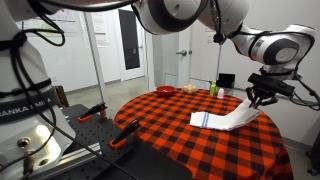
\includegraphics[width=3.80cm]{figures/generated/literature_review/point_observation_v1.jpg}};
  \node[lpPhoto] at (0.55,3.42)
    {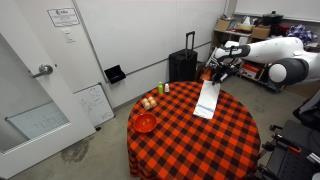
\includegraphics[width=3.80cm]{figures/generated/literature_review/point_observation_v2.jpg}};
  \draw[draw=black!55,line width=0.4pt] (0.55,3.5625) rectangle (4.35,5.70);
  \draw[draw=black!55,line width=0.4pt] (0.55,1.2825) rectangle (4.35,3.42);
  \draw[lpFrame] (0.35,0.35) rectangle (4.55,0.98);
  \node at (2.45,0.665) {给定机器人点流 $a_{0:T}$};
  \draw[lpArrow] (4.86,3.10) -- (5.34,3.10);

  \node[lpPhoto] at (5.55,5.55)
    {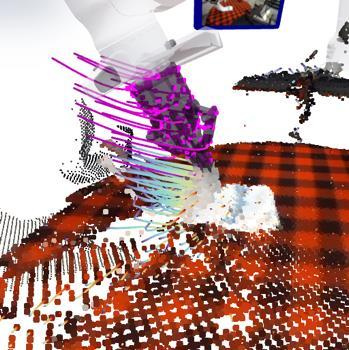
\includegraphics[width=4.65cm]{figures/generated/literature_review/point_prediction_1s.jpg}};
  \node[lpPhoto] at (11.10,5.55)
    {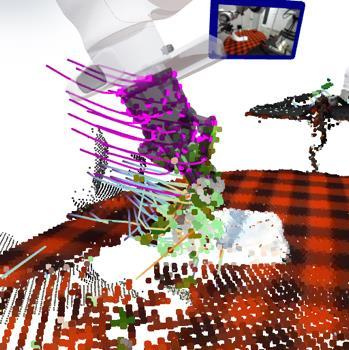
\includegraphics[width=4.65cm]{figures/generated/literature_review/point_reference_1s.jpg}};
  \draw[draw=black!55,line width=0.4pt] (5.55,0.90) rectangle (10.20,5.55);
  \draw[draw=black!55,line width=0.4pt] (11.10,0.90) rectangle (15.75,5.55);
  \node at (7.875,0.53) {$t_0+1.0\,\mathrm{s}$};
  \node at (13.425,0.53) {$t_0+1.0\,\mathrm{s}$};
\end{tikzpicture}
\endgroup
